\title{Multivariate Statistical Learning - A simple Anomaly Detection using K-means algorithm}
\author{
        Tommaso Puccetti \\
                Studente presso Universita degli studi di Firenze
}
\date{\today}
\documentclass[12pt]{article}
\usepackage[english]{babel}
\usepackage{graphicx}
\usepackage{hyperref}
\usepackage[procnames]{listings}
\usepackage{color}



\definecolor{keywords}{RGB}{255,0,90}
\definecolor{comments}{RGB}{0,0,113}
\definecolor{red}{RGB}{160,0,0}
\definecolor{green}{RGB}{0,150,0}

\lstset{language=Python, 
	backgroundcolor=\color{yellow},
	basicstyle=\fontsize{2}{4}\selectfont\ttfamily\scriptsize, 
	keywordstyle=\color{keywords},
	commentstyle=\color{comments},
	stringstyle=\color{green},
	showstringspaces=false,
	identifierstyle=\color{black},
	procnamekeys={def,class},
}
	

\begin{document}
\maketitle
\tableofcontents
\listoffigures

\section{Clustering: basics}
	Clustering analysis \textit{is a collection of statistical methods that can be used to assign units
	to groups, where group members share some characteristic}. Possible usage are: 
	
	\begin{itemize}
		\item \textbf{data reduction}: reduce data that are homogeneous (similar);
		\item \textbf{find “natural clusters”} and describe their unknown properties;
		\item \textbf{find} useful and suitable \textbf{groupings};
		\item \textbf{find} unusual data objects (i.e. outlier detection).
	\end{itemize}

	The aim is to find a way of \textbf{grouping statistical units} (or variables) in a data
	set in such a way that:
	\textbf{units are similar within groups and dissimilar among groups}. 
	
	\subsection{Main steps}
		
		The essentials steps for a clustering algorithm are the following:
		
		\begin{enumerate}
			\item \textbf{Define a metric} to evaluate distances between units;
			\item \textbf{Define an algorithm} to form groups. 
		\end{enumerate}
	
		The grouping algorithm can be:
		
		\begin{itemize}
			\item Hierarchical;
			\item Non-hierarchical.
		\end{itemize}
	
\section{Non-hierarchical clustering: K-means}
	K-means clustering is one of the simplest and popular unsupervised machine learning algorithms. The aim is to find a partition of the dataset into a set of K clusters. To achieve that the algorithm takes a given K and then find a partition of K clusters that optimizes the chosen partitioning criterion. Here the main steps in details:
	\begin{enumerate}
		\item choose K points at random as cluster centers
		(centroids);
		\item assign each unit to its closest centroid,
		using an opportune distance measure (usually Euclidean or Manhattan);
		\item calculate the centroid of each cluster and use it as
		the new cluster center;
		\item go back to step 2, stop when cluster centers
		do not change any more.
	\end{enumerate}

	\subsection{K-means: implementation}
		The implementation of the algorithm can be found in the \textbf{\textit{skmeans.py}} file. The file contains \textbf{K\_means} class declaration wich implements the \textbf{\textit{fit()}} method, used to find the centroids of the dataset, given K. The class also implements all the methods necessary to use K-means in the context of an anomaly detection algorithm. These methods are explained in details in the anomaly detection section.\\
		\begin{enumerate}
			\item First of all the algorithm choose K random centroid.
				\begin{lstlisting}
z = self.rng.permutation(len(X))[:self.k]
X = np.array(X, dtype= "float64")
centers = X[z]
				\end{lstlisting}
			\item The second step of the fit() method is to \textbf{calculate the} \textbf{Euclidean distance} between all the dataset points in respect to the K centroids. The distances are used to assign all the points to the nearest cluster, using K labels. 
			$$d(x,y) = \sqrt[2]{\sum_{i=0}^n (x_{i} - y_{i})^{2}} $$
				\begin{lstlisting}
for i in range(self.k):
	distances[:,i] = np.linalg.norm(X - centers[i], axis=1)	
			
labels= np.argmin(distances, axis = 1)
				\end{lstlisting}
			
			\item For each cluster the algorithm \textbf{calculates the new centroid} as the mean of the points assigned to them:
			
				\begin{lstlisting}
for i in range(self.k):
	if(i in labels):
		new_centers = X[labels == i].mean(0)
		center_temp.append(new_centers)
	else:
		center_temp.append(self.farthest(X, distances, labels))
		
new_centers = np.array(center_temp, dtype= "float64")
					
				\end{lstlisting}
				This phase could generate an error in case one of the centroid has no segments assigned: in fact the computation of the mean for the centroid could not be done, as we try to divide for zero. To avoid that, the \textbf{\textit{farthest()}} function is used to choose the farthest segment from the centroid, designating it as the new centroid.
				
				\begin{lstlisting}
def farthest(self, segments, distances, labels):
	counts = np.bincount(labels)
	new_centroid_idx = np.argmax(distances[:, np.argmax(counts)],
		axis =0)
	new_centroid = segments[new_centroid_idx]
	print(new_centroid)
								
	return new_centroid	
				\end{lstlisting}
				 
			\item Repeats from point 2 to point 3 until the new centroids are equal to the centroids from the previous step.
			\begin{lstlisting}
if np.all(centers == new_centers):
	break

centers = new_centers
			\end{lstlisting}
			
		\end{enumerate}
	
		

	
		The \textbf{\textit{kmeans\_sk.py}} file contains an example of usage for the algorithm. The dataset presents 4 distinct points aggregates. Using the \textbf{\textit{fit()}} method with $K = 4$ the algorithm, as we expected, identifies the 4 aggregates of points as 4 clusters.
		
		\begin{figure}[h!]
			\centering
			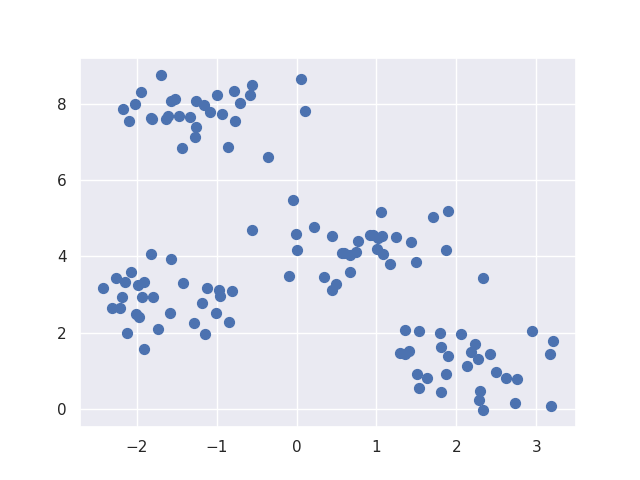
\includegraphics[scale=0.60]{img/points.png}
			\label{fig1}
			\caption{Example of K-means usage on artificial data. }
		\end{figure}
	
		\begin{figure}[h!]
			\centering
			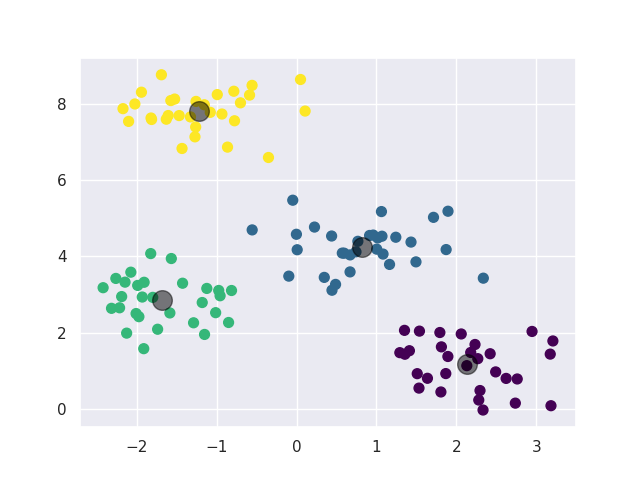
\includegraphics[scale=0.60]{img/points_centroid.png}
			\label{fig2}
			\caption{Example of K-means usage on artificial data: output.}
		\end{figure}
\newpage
		
\section{Anomaly detection using K-means}
	Assume to have a record of how some values changes over time (i.e server usage, heartbeat data ecc), also assume this record having a regular shape or pattern that is indicative of some kind of "normal" behaviour. The K-means algorithm can be used to spot anomalies given the normal behaviour. The waveform in \textit{Figure 3}  rapresents a noise that is regular over time, instead, in \textit{Figure 4}, an example of a possible anomaly is introduced.
	
	\begin{figure}[h!]
		\centering
		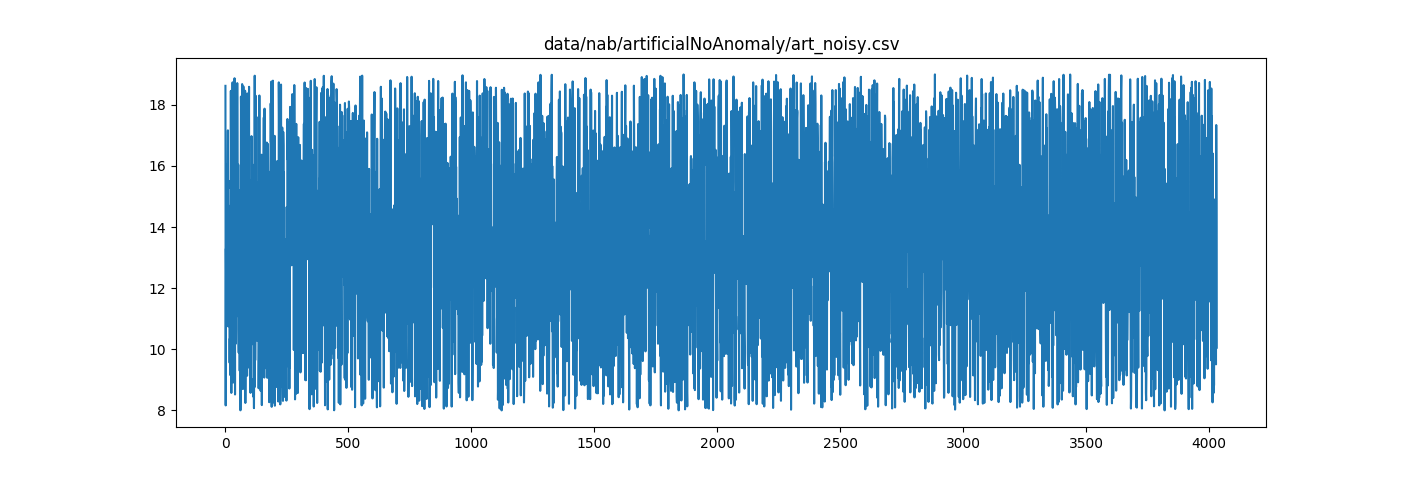
\includegraphics[scale=0.40]{img/normalbe.png}
		\label{fig3}
		\caption{Noise dataset without anomaly.}
	\end{figure}
	
	\begin{figure}[h!]
		\centering
		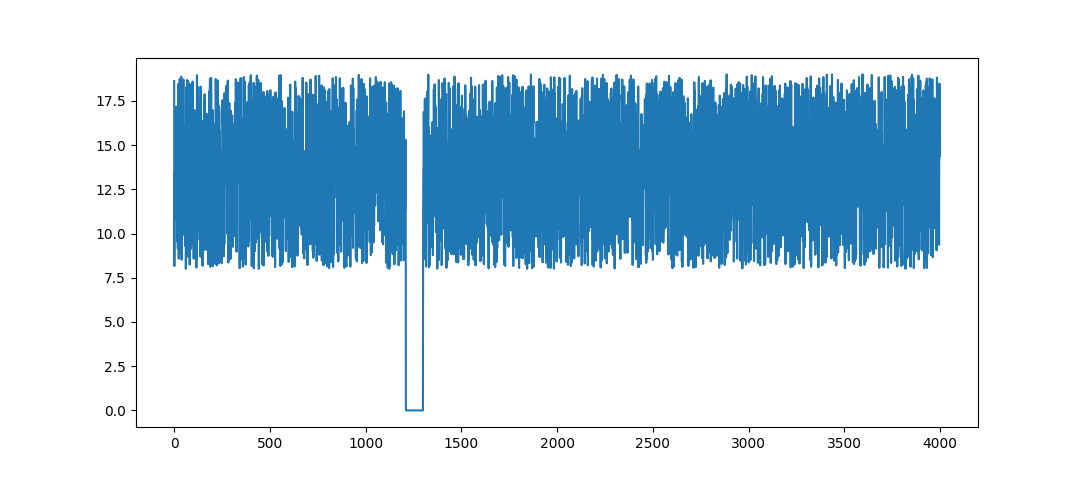
\includegraphics[scale=0.515]{img/anomaly.png}
		\label{fig4}
		\caption{Noise dataset with an anomlay.}
	\end{figure}


	The idea is the following:
	\begin{enumerate}
		\item split the waweform into \textbf{\textit{n}} segments of length \textbf{\textit{l}}: every segment is considered a statistical unit;
		\item apply the K-means algorithm over the l-dimension points obtained (segments). The results are K cluster's \textit{centroids};
		\item a centroid is a segments itself that can be used to reconstruct the original waweform: for every segments the nearest centroid is used to approximate the current;
		\item once obtained a recostructed waweform using only centroids, we can subtract it from the original: the result is also a waweform that rapresents the noise signal between the two;
		\item the last step is to use a treshold value to detect where the error between the original and the reconstructed waweforms is anomalous in respect to the noise obtained. 
	\end{enumerate}

	\subsection{Implementation}
		
		\subsubsection{Segmentation}
			The first step is to define a training set. The training set is a wafeform wich represents the normal behaviour for our dataset. Is obvious that, more we know about the normal behaviour, more we are capable to spot anomalies. The training set, once splitted in segments, will be used as input for K-means algorithm. The segmentation is done using the \textit{\textbf{segmentation()}} function implemented in the K-means class.
			
			\begin{lstlisting}
segment_len = 32
slide_len = 16
km = skmeans.K_means(30)
segments = km.segmentation(train_array, segment_len, slide_len)
			\end{lstlisting}
			
			The idea is to have a sliding window wich is traslated to obtain overlapping segments.
			This function simply takes the training set as input, along with the desired length for the segments and the slide length for the window. The slide length is choosen to be the half of the segments length, this way the reconstruction could be easily done in further steps. The output would be a Numpy's array containing n segments. The dataset, shown in picture from now on, refers to Amazon server CPU usage with a known anomaly.
			
			\begin{figure}[h!]
				\centering
				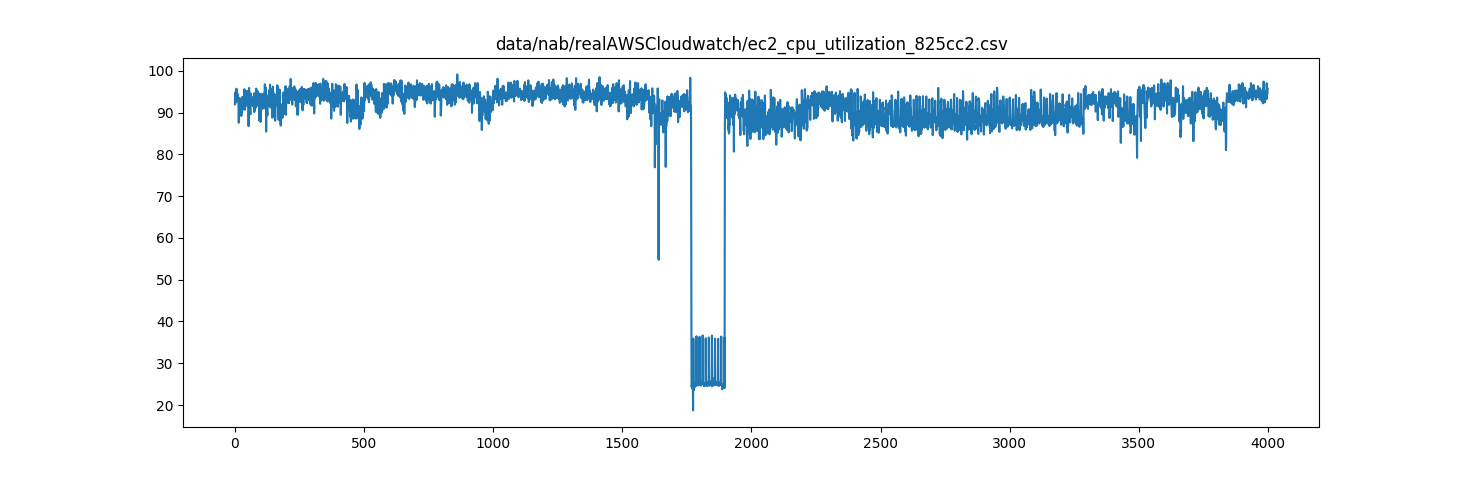
\includegraphics[scale=0.40]{img/dataset.png}
				\label{fig5}
				\caption{Amazon's server CPU usage with a known anomaly }
			\end{figure}
			
		\subsubsection{Calculate centroids}
		
			The \textbf{\textit{fit()}} function of the K-means class, described in the previous chapter, is used to calculate the centroid given the segments obtained from the previous step.  
			\begin{lstlisting}
centr = km.fit(segments)
learn_utils.plot_waves(centr, step=3)
			\end{lstlisting}	
			The output would be a Numpy's array containing K centroids of the dataset. The picture below shows some of the normal waweform obtained.
			
			\begin{figure}[h!]
				\centering
				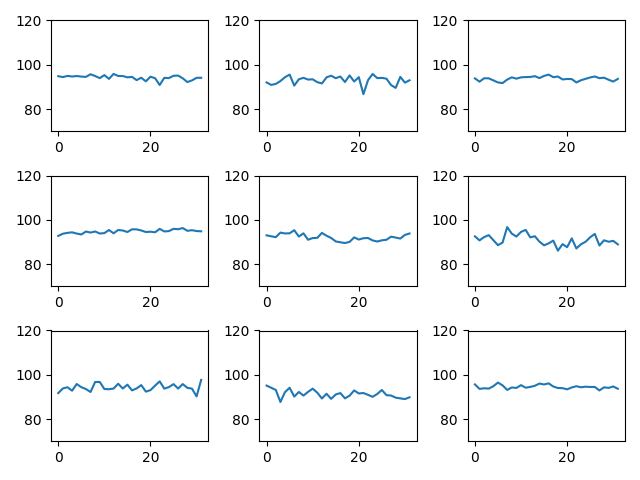
\includegraphics[scale=0.60]{img/centroids.png}
				\label{fig6}
				\caption{Centroids obtained using K-means algorithm}
			\end{figure}
		
		\subsubsection{Reconstruction}
		
			Once obtained the centroids we can use them to reconstruct the original waweform. First of all we have to apply again the segmentation process, this time over the entire dataset. Then the \textbf{\textit{predict()}} function is used to find, for all the segments obtained, the nearest centroid. The output would be an array wich store in the n-th position a label referring to the nearest centroid for the n-th segment.
		
			\begin{lstlisting}
segments = km.segmentation(dataset_array, segment_len, slide_len)
lab = km.predict(centr, segments)
			\end{lstlisting}  
			
			\begin{lstlisting}
def predict(self, centers, windowed_segments):
	distances = np.zeros((len(windowed_segments), self.k))
	for i in range(self.k):
		distances[:,i] = np.linalg.norm(windowed_segments 
			- centers[i], axis=1)
		
	labels= np.argmin(distances, axis = 1)
	print("Predicted Labels")
	print(labels)
				
	return labels
			\end{lstlisting}
		
			\begin{lstlisting}
Predicted Labels
[12 27  3 14 23 22 27 16 12 26 12 19  4  5  7  6  6  6 28 10  9  1 10  4
29 16  6 21 20 15 13  9 24  7 12  2 17 17 11  1 23  9 10  9 11 11 10  6
6  8  0  8  9  9  1 11  0 23  0 21 26 27  6  8 24 23 25 25 10 23 25  8
9 10 25  1 11 10  5 23 24  0 10  8  9 10 23 23  0 23 23 18 10 10  7 23
6  5 23  7 21 26 21 15 13 27 14 27 14 21 15 15 15 15 15 15 15 13 13 21
20 12 15 26 26 20 15 15 26 15 26 15 15 21 26 21 26 27 27 12 27 27 23 27
27 21 26 27 21 21 20 15 26 21 26 26 15 27 15 21 26 26 21 15 21 21 26 26
21 26 26 15 15 26 21 21 26 21 21 26 21 21 26 21 15 26 21 15 26 21 15 21
20 21 26 21 26 26 21 21 26 21 21 26 20 27  6  7 27 12 27 14  6 21 21 15
21 13 13 27  6 10  0 23  9  0 12 21 12 12 20 20 27 12 27 12 27 21 21 20
23 23  9  0  9 10 10  8  9]
			\end{lstlisting}
			
			Finally the reconstruction algorithm is used to obtain the whole waweform. 
		
			\begin{lstlisting}
noise = detection.reconstruction(dataset_array, segments, lab, 
	centr, slide_len, segment_len)
			\end{lstlisting}
				
			\begin{lstlisting}
def reconstruction(data, segments, label, centroid, slide_len, segment_len):
	n = 0
	reconstruction = np.zeros(len(data)) 
	win_seg = np.zeros(len(data)) 
	pos = 0
	for segment in segments:
		nearest_centroid = centroid[label[n]]
		win_seg[pos:pos+segment_len] += segment
		reconstruction[pos:pos+segment_len] += nearest_centroid
		pos = n * slide_len
		n = n + 1

	noise = reconstruction[0:len(reconstruction)] -
		win_seg[0:len(win_seg)]
	n_plot_samples = len(noise)

	plt.plot(win_seg[0:n_plot_samples], label="Original waveform")
	plt.plot(reconstruction[0:n_plot_samples], 
		label="Reconstructed waveform")
	plt.plot(noise[0:n_plot_samples], label="Noise")
	plt.legend()
	plt.show()
	plt.hist(noise)
	plt.show()

	return noise, np.mean(noise)
			\end{lstlisting}
		
			The noise obtained as output is ploted along with the original and the reconstructed waweform.
		
			\begin{figure}[h!]
				\centering
				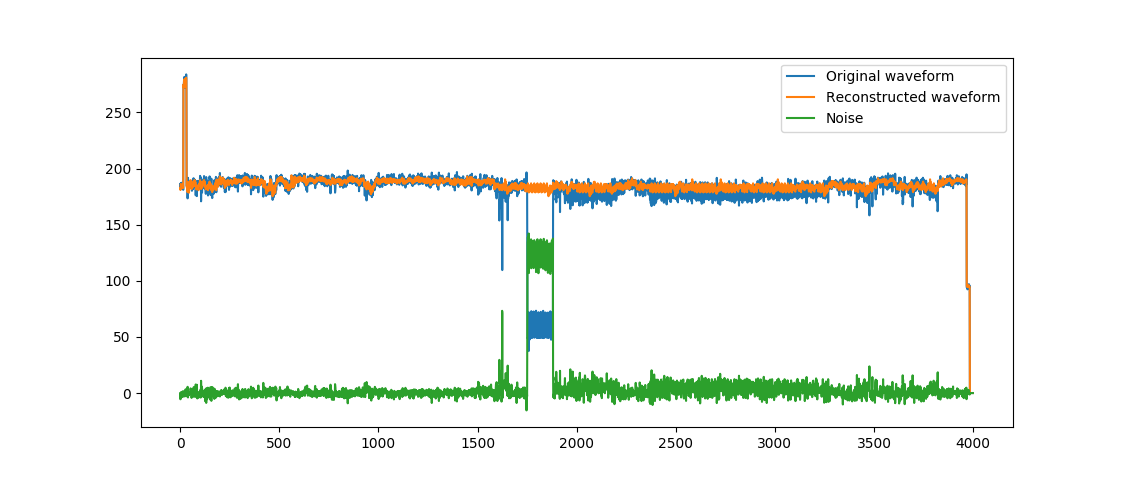
\includegraphics[scale=0.550]{img/noise.png}
				\label{fig7}
				\caption{Noise signal.}
			\end{figure}
	\newpage	
		\subsubsection{Detecting anomalies}
			The noise obtained from previous step can be analized to detect anomalies. To do that we defined the noise signal as being normally distributed with a mean of zero. If it suddenly changes into another distribution, something unusual or anomalous is happening. To spot outliers values in the noise distribution we use a treshold value defined as:
			
			$$ mean \pm 4*std $$
			
			Based on the normal distribution properties, values lower than $mean – 4 * std$ deviation and higher than $mean + 4 * std$ should be extremely rare and could be considered as an anomaly: 
			\begin{itemize}
				\item $68\%$ of all values fall between $[mean-\sigma; mean+\sigma]$;
				\item $95\%$ of all values fall between $[mean-2*\sigma; mean+2*\sigma]$; 
				\item $99,7\%$ of all values fall between $[mean-3*\sigma; mean+3*\sigma]$ 
			\end{itemize}
		
			These 3 rules are also known as the $68 \_–95 \_–99.7$ rule.
			
			\begin{figure}[h!]
				\centering
				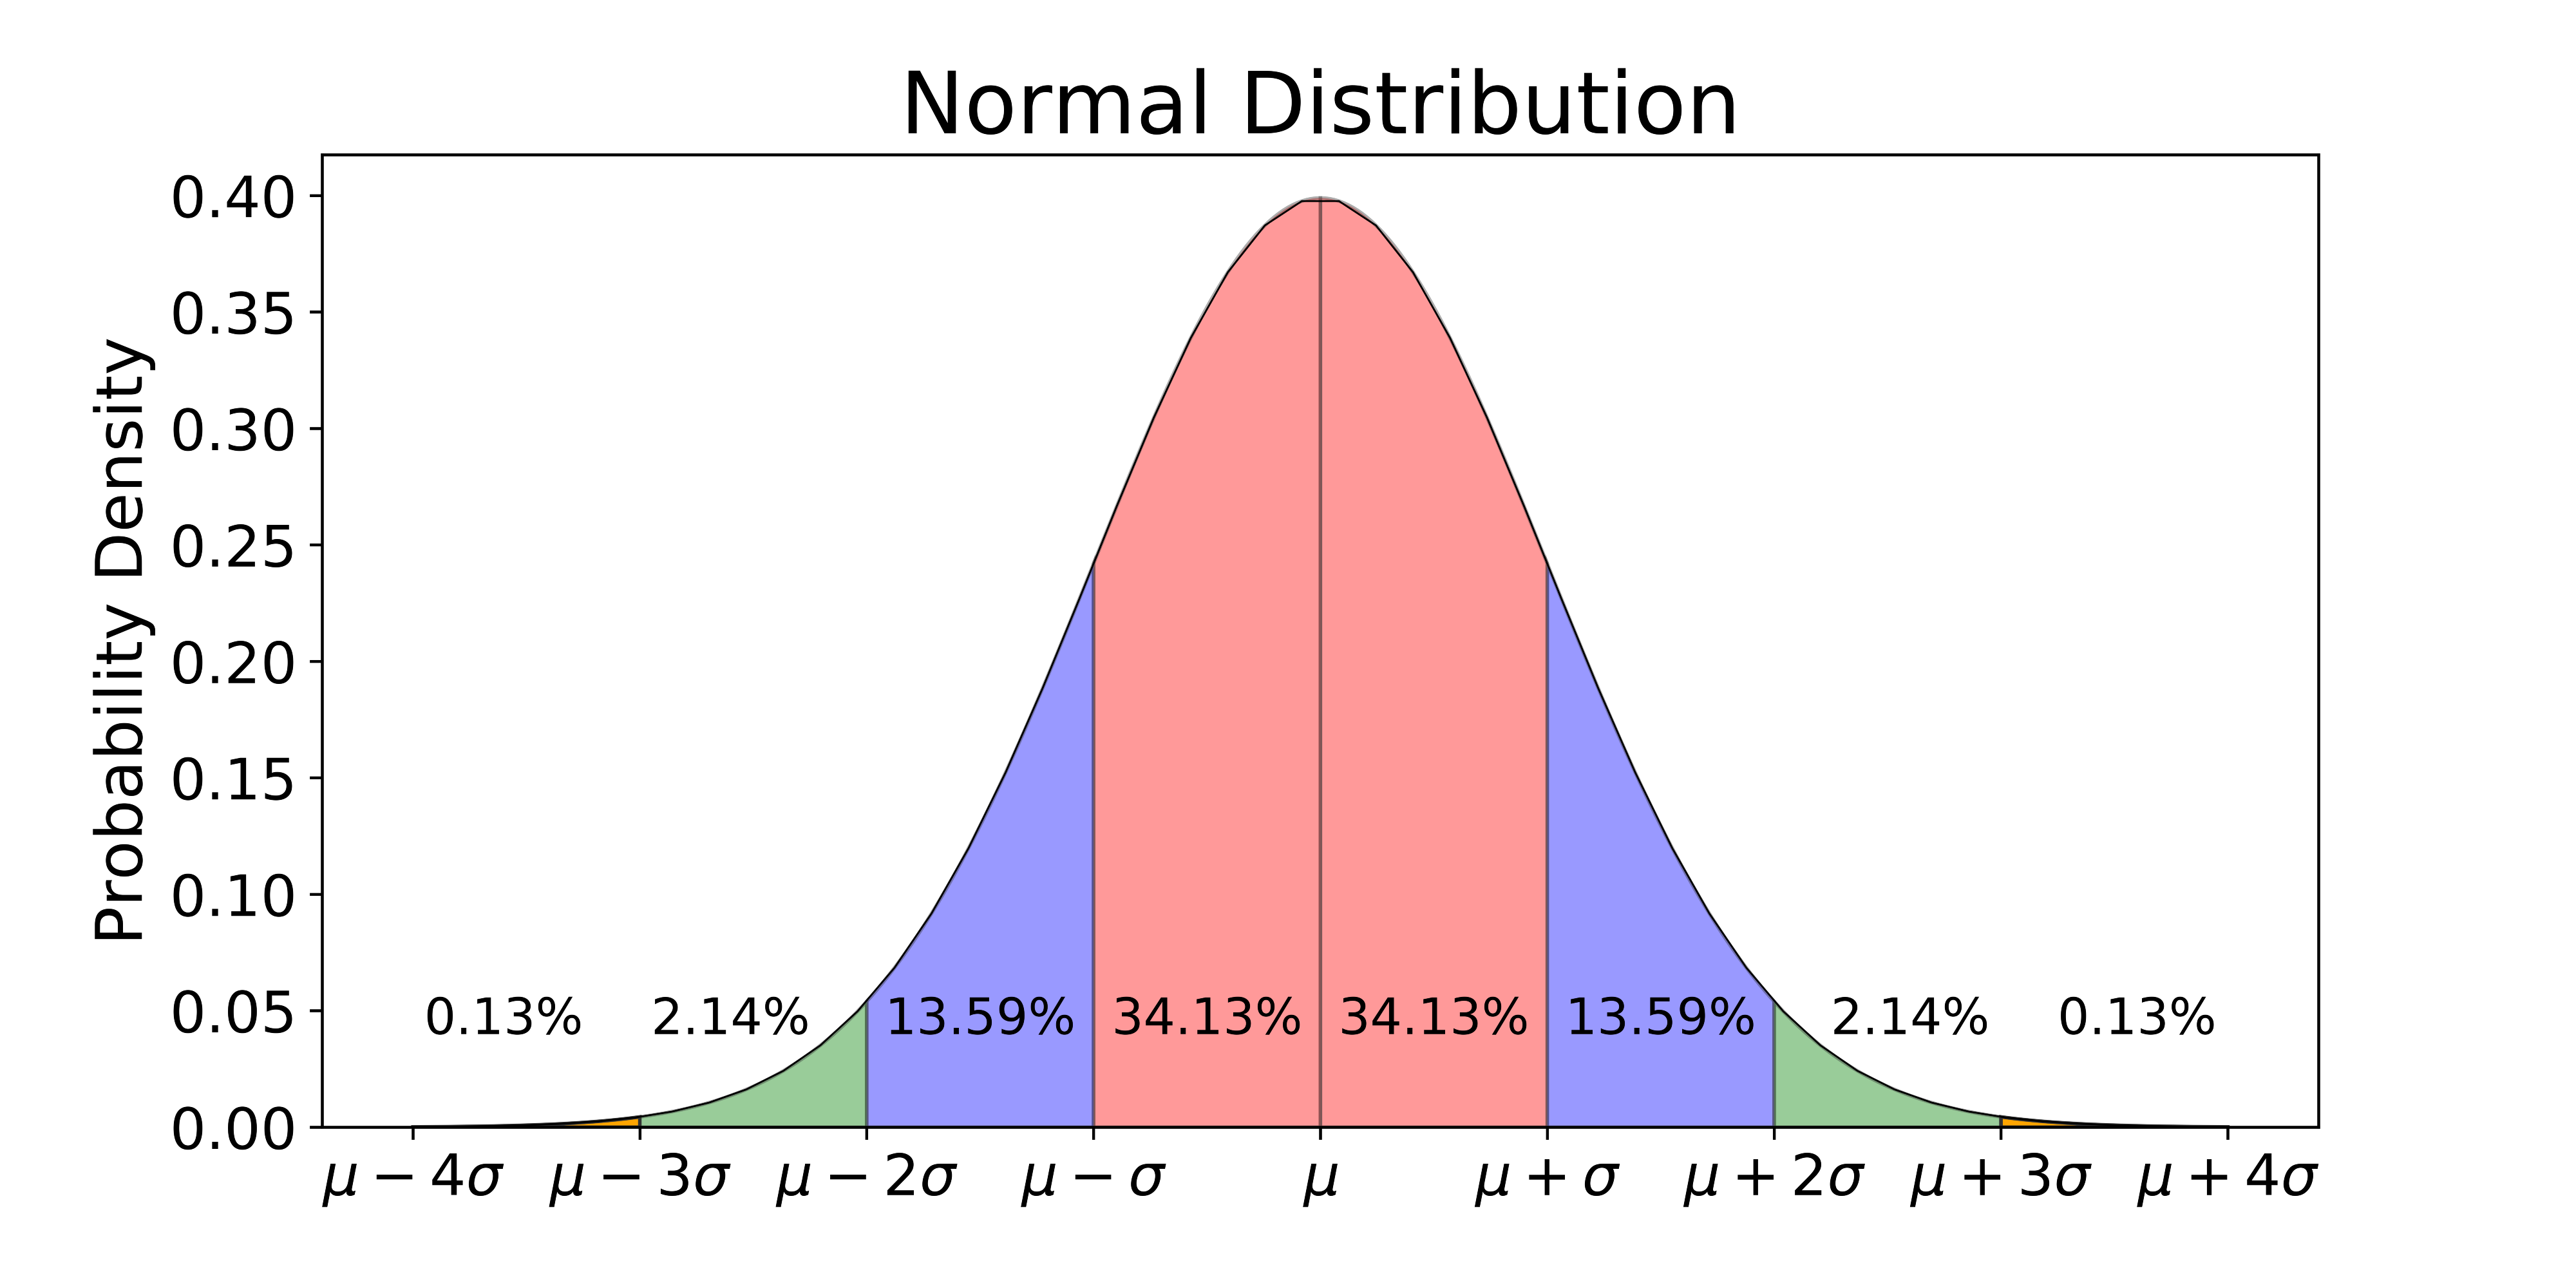
\includegraphics[scale=0.1]{img/rule.png}
				\caption{$68 \_–95 \_–99.7$ rule.}
			\end{figure}
			
			\begin{lstlisting}
pos_treshold = np.mean(noise) + coef * np.std(noise)
neg_treshold = np.mean(noise) - coef * np.std(noise)
anomalies = []

for i in range(0,len(noise)):
	if(noise[i] <= neg_treshold):
		anomalies.append((i,noise[i]))
	if(noise[i] > pos_treshold):
		anomalies.append((i, noise[i]))
			\end{lstlisting}
			
			The \textit{if} branches are used to detect and store anomalies in a specific Python list, returned as output of the function. 
			
			\begin{lstlisting}
[[1752.     136.241]
[1753.     136.351]
[1754.     137.356]
[1755.     137.524]
[1756.     131.364]
[1757.     132.855]
[1758.     141.735]
[1759.     106.452]
[1760.     132.65 ]
[1761.     134.158]
	.
	.
	.
[1875.     133.178]
[1876.     127.938]
[1877.     135.216]
[1878.     135.596]
[1879.     109.638]
[1880.     136.132]]
			\end{lstlisting}
			
		\subsubsection{Conclusion}
			The first part of the code (noise production) can be used as base to implement an anomaly detection wich use different approach for detection. For example, a sliding window can be used to detect changes in the noise distribution rather then use a treshold value to detect outliers values. The idea is to use window containing the n most recent elements. If the mean and standard derivation of this window change too much from their expected values, we can deduce an anomaly. The use of the sliding windows could be combined with the outliers detection to improve the detection precision.
			
			\begin{figure}[h!]
				\centering
				
\includegraphics[scale=0.08]{img/github.png}
			\end{figure}
			The code of the project can be reached at: \href{https://github.com/GeorgeSmiley/masl}{https://github.com/GeorgeSmiley/masl}.
		\subsubsection{Dataset}
		
			The dataset used is the Numenta Anomaly Benchmark (NAB) that is a benchmark for evaluating algorithms for anomaly detection in streaming and online applications. It is comprised of over 50 labeled real-world and artificial timeseries data files plus a novel scoring mechanism designed for real-time applications. All of the data and code is fully open-source, with extensive documentation, and a scoreboard of anomaly detection algorithms: \href{github.com/numenta/NAB}{github.com/numenta/NAB}.
			
	
		
			 
		
		
		

		
	
	
	
	
	
	
	
	
	
	
	
	
	
	
	
	
	
	
	
	
	
	
\end{document}